\section{Methodology}

\begin{wrapfigure}{r}{0.55\textwidth}
\vspace{-2.7cm}
\begin{minipage}{0.55\textwidth}
\centering
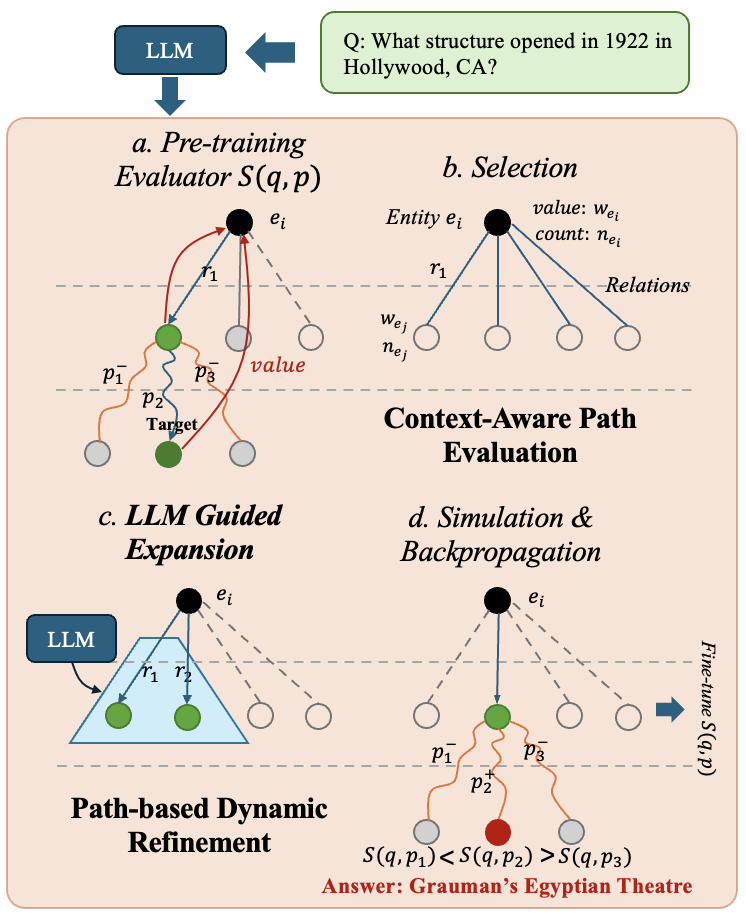
\includegraphics[scale=0.56]{figure/framework.png}
% \vspace{-0.6cm}
\caption{Overview of \method{}. The reasoning process begins with an MCTS guided by an LLM-based planner, which selects top-$k$ semantically relevant relations at each expansion step. A context-aware path evaluator scores each candidate path during simulation. To enable continual adaptation, high-confidence pseudo-paths generated during search are used to dynamically fine-tune the evaluator.}
\label{framework}
\vspace{-1.4cm}
\end{minipage}
\end{wrapfigure}

% \begin{figure}[t!]
%   \centering
%   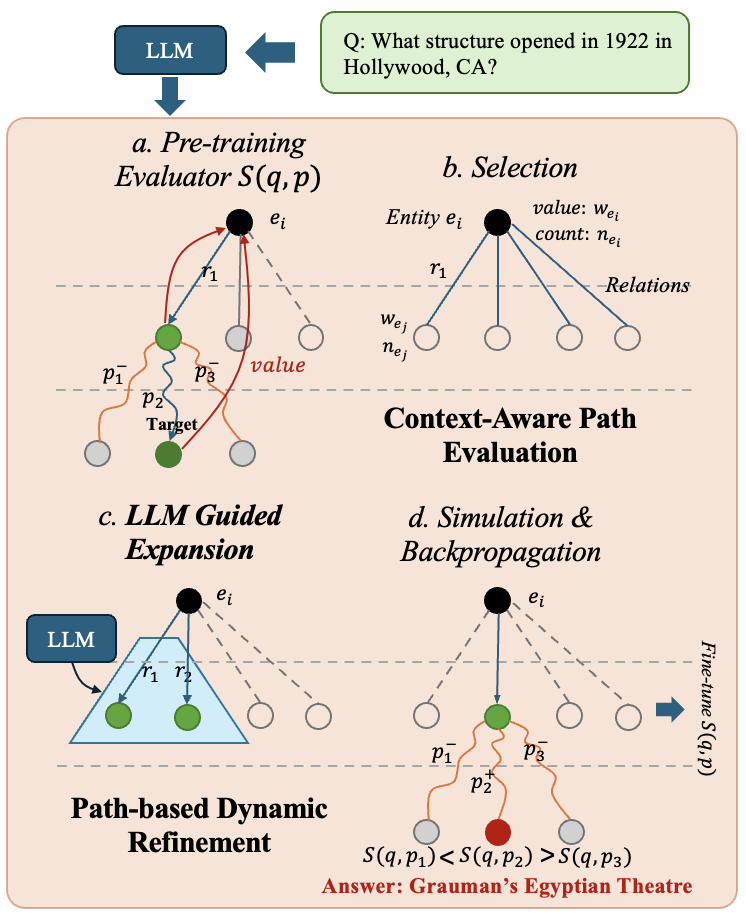
\includegraphics[width=0.48\textwidth]{figure/framework.png} 
%   % \vspace{-0.1cm}
% \caption{Overview of \method{}. The reasoning process begins with an MCTS guided by an LLM-based planner, which selects top-$k$ semantically relevant relations at each expansion step. A context-aware path evaluator scores each candidate path during simulation. To enable continual adaptation, high-confidence pseudo-paths generated during search are used to dynamically fine-tune the evaluator.}
%   \label{framework}
%   % \vspace{-0.4cm}
% \end{figure}

\subsection{Problem Formulation}

We define Knowledge Graph Question Answering (KGQA) as the task of answering a natural language question by reasoning over a knowledge graph (KG). The KG is typically represented as a set of triples $\mathcal{K} = \{(e_s, r, e_o) \} \subseteq \mathcal{E} \times \mathcal{R} \times \mathcal{E}$, where $\mathcal{E}$ and $\mathcal{R}$ denote the sets of entities and binary relations.
The goal of KGQA is to find a set of answers $\mathcal{A}_q \subseteq \{(e_1,r_1,e_2), (e_2,r_2,e_3)\cdots\} $ for question $q$, such that a reasoning path through the KG leads from a topic entity to the correct answer. Formally, this is often framed as mapping $q$ to an executable query program $p_q$, where $\text{LLM}(p_q|{\mathcal{K}}) = \mathcal{A}_q$.

\subsection{Overview of Framework}
In this paper, we propose a dynamically adaptive reasoning framework \method{} for KGQA, as shown in Fig.~\ref{framework}. 
\method{} comprises three components: (1) \textbf{LLM Guided Expansion.} \method{} employs MCTS to incrementally expand reasoning paths, guided by an LLM-based planner that proposes relevant relations. This reduces computational overhead and enhances efficiency in KG exploration; (2) \textbf{Context-Aware Path Evaluation.} To capture the evolving semantics of reasoning paths, \method{} employs a lightweight Transformer-based scorer with cross-attention to jointly encode the question and path embeddings. This enables context-sensitive evaluation and improves the accuracy and relevance of multi-hop reasoning; (3) \textbf{Path-based Dynamic Refinement.} \method{} uses intermediate paths from MCTS as dynamic pseudo-paths to iteratively fine-tune the path evaluator, enhancing its ability to capture question-specific semantics and improving reasoning accuracy.


\subsection{LLM Guided Expansion}

A key challenge in KGQA is efficiently exploring the vast search space of multi-hop reasoning paths, especially under weak or no supervision. Existing methods often struggle to balance search efficiency and semantic relevance, resulting in either redundant exploration or missed correct paths~\citep{long2025enhancing,li2024simple}. To address this, the LLM-Guided Expansion module employs MCTS~\citep{kocsis2006bandit} as the backbone for symbolic path expansion. At each step, an LLM proposes semantically relevant relations, narrowing the search space and improving path quality, while MCTS ensures a balanced trade-off between exploration and exploitation.

% At each step, an LLM-based planner proposes top-$k$ semantically relevant relations based on the current state and the question. MCTS incrementally expands paths and selects promising candidates through simulation and backpropagation, enabling scalable and focused search aligned with the question intent.

% The core of path expansion in \method{} lies in selecting relations relevant to the question $ q $ for further expansion. For reducing computational costs and enhancing efficiency in large-scale knowledge graph exploration, we introduce an LLM-based planner to select the top-k relevant relations for path expansion in the proposed \method{}. 
Specifically, each node in the MCTS represents a reasoning state anchored at a specific entity in the KG. Given the current state, possible actions correspond to selecting an outgoing relation to extend the reasoning path. During the \textbf{Selection} phase, the search traverses from the root to a leaf node by recursively choosing children with the highest Upper Confidence Bound for Trees (UCT) score~\citep{kocsis2006bandit}, which is defined as:
\begin{equation}
\label{selection}
UCT = \frac{w_i}{n_i} + C \sqrt{\frac{\ln N}{n_i}},
\end{equation}
where $w_i$ denotes the accumulated reward of node $i$, $n_i$ its visit count, $N$ the visit count of its parent, and $C$ a constant that balances exploration and exploitation. This criterion guides the search to trade off between exploring new relations and exploiting promising paths.
In the \textbf{Expansion} phase, the selected leaf node is expanded by retrieving the outgoing relations of its entity $e_i$, denoted as $\mathcal{R}_{e_i} = \{r_1, r_2, \dots, r_n\}$. To avoid exhaustive branching, we prompt an LLM with the question $q$ and candidate relations $\mathcal{R}_{e_i}$, selecting the top-$k$ relations most semantically aligned with $q$:
\begin{equation}
\mathcal{R}_{top-k} = \text{LLM}(q, \mathcal{R}_{e_i}).
\end{equation}
These top-$k$ relations are then used to generate new child nodes, ensuring that expansion favors semantically meaningful directions and remains computationally efficient.

% Given a node in the MCTS representing a relation $ r \in \mathcal{R} $, we first retrieve all entities $ e \in \mathcal{E} $ that are connected to this relation $ r $ as the tail entities $ T_r = \{e_1, e_2, \dots, e_n\} $. Then, for each tail entity $ e_i $, we retrieve all relations $ \mathcal{R}_i $ associated with $ e_i $, forming a new set of candidate relations $ \mathcal{R}_{cand} = \bigcup_{e_i \in T_r} \mathcal{R}_i $. These candidate relations are used for expanding the reasoning path. To guide this selection efficiently, we employ an LLM to choose the top-k relations that are most relevant to the question $ q $, based on the current reasoning context. The LLM takes as input the question $ q $ and the set of candidate relations $\mathcal{R}_{cand}$, and outputs the top-k relations $ \mathcal{R}_{top-k} $ most aligned with $ q $:
% \begin{equation}
% \mathcal{R}_{top-k} = \text{LLM}(q, \mathcal{R}_{cand})
% \end{equation}
% This method ensures that only the most relevant relations are considered for path expansion, thereby improving computational efficiency and steering the search toward the correct answer.

\subsection{Context-Aware Path Evaluation}

While LLM-guided expansion effectively narrows the search space by selecting semantically relevant relations, it does not ensure that all expanded paths remain valid in the broader reasoning context. As the search progresses, path semantics evolve dynamically, and early promising trajectories may later become misleading or irrelevant. Prior works attempt to filter or pre-plan paths to improve relevance~\citep{fang2024karpa,long2025eperm}, but still leave gaps in capturing evolving path semantics during search. To address this, we integrate a lightweight Transformer-based path scorer into MCTS’s simulation phase, employing cross-attention to jointly encode the question and current path, enabling adaptive evaluation that reflects evolving semantics.

% While LLM-guided expansion effectively narrows the search space by selecting semantically relevant relations, it cannot guarantee that expanded paths remain valid or meaningful in the broader reasoning context. As the search progresses, path semantics evolve dynamically, and trajectories that appear promising early may later become irrelevant or misleading~\citep{sun2018open,ye2022routing}. To address this, Context-Aware Path Evaluation integrates a lightweight Transformer-based path scorer into the simulation phase of MCTS. This scorer leverages cross-attention to jointly encode the question and the current reasoning path, allowing for adaptive evaluation that captures evolving semantics. By assigning scores to simulated paths based on question-path alignment, this module enables more accurate path ranking throughout the search process.

\textbf{Context-Aware Path Evaluator.} 
In the \textbf{Simulation} phase, we assess the quality of candidate paths generated during MCTS rollouts. Given a question $q$ and a candidate relation path $p_r = (r_1, r_2, \ldots, r_l)$, where $p_r$ is formed by sequentially selecting relations during expansion, both $q$ and $p_r$ are first encoded using a pre-trained LLM. Let $\mathbf{z}_q \in \mathbb{R}^d$ denote the embedding of $q$ and $\mathbf{z}_{r_i} \in \mathbb{R}^d$ the embedding of relation $r_i$. To capture the sequential structure of $p_r$, we introduce a learnable positional encoding $\mathbf{e}_i^{\text{pos}}$ for each relation. The final input sequence is obtained by combining $\mathbf{z}_{r_i}$ with $\mathbf{e}_i^{\text{pos}}$ and feeding the sequence into a Transformer encoder:
\begin{equation}
\mathbf{E}_{p_r} = \text{Transformer}([\mathbf{z}_{r_1} + \mathbf{e}_1^{\text{pos}}, \ldots, \mathbf{z}_{r_l} + \mathbf{e}_l^{\text{pos}}]),
\end{equation}
where $\mathbf{e}_i^{\text{pos}} = \mathbf{E}^{\text{pos}}[i]$ is the positional embedding of the $i$-th hop, drawn from a trainable matrix $\mathbf{E}^{\text{pos}} \in \mathbb{R}^{L \times d}$, where $L$ is the maximum path length and $d$ the embedding dimension. To further incorporate question-specific information, we apply a cross-attention mechanism, allowing the encoded path representation $\mathbf{e}_{p_r}$ to attend to the question embedding $\mathbf{z}_q$:
\begin{equation}
\mathbf{H} = \mathbf{E}_{p_r} + \mathrm{CrossAttn}(\mathbf{E}_{p_r}, \mathbf{z}_q),    \;
% \end{equation}
% \begin{equation}
    with\; \text{CrossAttn}(\mathbf{E}_{p_r}, \mathbf{z}_q)=\text{softmax}({\mathbf{E}_{p_r} \cdot \mathbf{z}_q^T}/{\sqrt{d_k}}) \cdot \mathbf{z}_q. 
\end{equation}
We then apply attention pooling over the relation representations $\mathbf{H}$ to obtain the hidden state of the relation path:
\begin{equation}
\mathbf{s}_{p_r} = \sum_{i=1}^l \alpha_i \textbf{h}_i, \quad \alpha = \text{Softmax}\big(\text{MLP}(\mathbf{H})\big),    
\end{equation}
where $\mathbf{h}_i$ is the hidden state of the $i$-th relation and $\alpha_i$ its learned attention weight. This pooling allows the model to emphasize informative steps along the reasoning path. The pooled path representation $\mathbf{s}_{p_r}$ is then concatenated with the question embedding $\mathbf{z}_q$, and the combined vector is passed through a multi-layer perceptron to compute the plausibility score of the question–path pair:
\begin{equation}
S(q, p_r) = \mathrm{MLP}\big([\mathbf{s}_{p_r}:\mathbf{z}_q]\big).    
\end{equation}
This context-aware evaluator assigns plausibility scores to partial reasoning paths by jointly encoding the question and relation sequence, providing accurate, context-sensitive guidance for MCTS.
% This context-aware evaluation model dynamically scores partial reasoning paths by jointly considering the question and the relation sequence, offering accurate and context-sensitive guidance to the MCTS search process.


\textbf{Pre-training of Evaluator.} To train the context-aware evaluator, we construct supervision by sampling positive and negative paths from local subgraphs. A path is positive if it links the head entity to a correct answer within a hop limit. Negatives come from two sources: hard negatives that terminate near but miss the answer, and random negatives from walks that avoid answer entities. Each training instance is a triplet $(q, p^+, p^-)$, with sequences zero-padded and masked for efficient batch training.

The model computes a plausibility score $S(q, p)$ for each question-path pair and is optimized using the Pair-wise Ranking loss~\citep{rendle2012bpr} to encourage higher scores for positive paths:
\begin{equation}
\label{pr}
    \mathcal{L}_{\text{PR}} = -\frac{1}{M} \sum_{i=1}^M \log \sigma\left( S(q, p^+_i) - S(q, p^-_i) \right),
\end{equation}
where $\sigma(\cdot)$ is the sigmoid function. This training strategy equips the evaluator with the ability to distinguish plausible reasoning paths, thereby improving the guidance signal during MCTS inference.
% Each training instance consists of a triplet $(q, p^+, p^-)$, where $p^+$ and $p^-$ are the positive and negative relation sequences, respectively. All relation sequences are zero-padded to a fixed maximum length $L$, and binary masks are generated to support efficient batch training. 

% Given a question-path pair $(q, p)$, let $S(q, p)$ denote the plausibility score computed by the evaluation model. The model is trained to discriminate positive paths from negative ones by minimizing the Bayesian Personalized Ranking (BPR) loss:
% \begin{equation}
% \mathcal{L}_{\text{BPR}} = -\frac{1}{N} \sum_{i=1}^N \log \sigma\left( S(q, p^+_i) - S(q, p^-_i) \right),    
% \end{equation}
% where $\sigma(\cdot)$ is the sigmoid function and $N$ is the batch size.

% To promote stable and effective learning, we ensure data deduplication for unique path sequences, dynamically balance the number of positive and negative samples, and utilize attention masking for variable-length paths during batch processing. This comprehensive training paradigm equips the model with the capacity to distinguish plausible reasoning paths from implausible ones, thereby providing a robust foundation for accurate and context-sensitive path evaluation during the search process.




\subsection{Path-based Dynamic Refinement}

While LLM-guided expansion and semantic scoring improve path exploration, the static evaluator may fail to generalize to the evolving search space. To address this, we introduce a dynamic refinement mechanism that leverages high-confidence paths from MCTS rollouts as pseudo-paths. 
These pseudo-paths serve as supervision signals, enabling continual adaptation of the evaluator to new reasoning contexts without requiring additional labeled data.
% These are used to incrementally fine-tune the evaluator, enabling it to adapt to new reasoning contexts and improve path selection without relying on additional supervision.

Specifically, during \textbf{Backpropagation} phase, the plausibility score estimated by the context-aware path evaluator is propagated along the visited nodes in the MCTS tree after each simulation. For every entity $e_i$ on the simulated path, we update its visit count and aggregated value as follows:
\begin{equation}
    n_{e_i}= n_{e_i} + 1, \quad w_{e_i}= \frac{\sum_j n_{e_j}\cdot w_{e_j}}{\sum_j n_{e_j}},
\end{equation}
where $n_{e_i}$ is the visit count and $w_{e_i}$ is the aggregated value of entity $e_i$. The value is computed as a weighted average over its child nodes $\{e_j\}$, and reflects the plausibility scores $w_{e_j}$ assigned during simulation. These updates refine the UCT estimates used in future selection steps, progressively biasing the search toward high-quality reasoning paths.

To construct supervision signals for fine-tuning, we dynamically sample pseudo-path pairs ($\hat{p}'_i$, $\hat{p}'_j$) from the set of explored paths during MCTS. Instead of relying on the evaluator’s predictions, we assign pseudo-labels based on empirically grounded values derived from the search process. Specifically, for entity $e_i$ along a reasoning path $p_r$, we define its search value as:
$w_{e_i} = \frac{w_{p_r}}{n_{e_i}}$,
where $w_{p_r}$ is the cumulative reward from all rollouts passing through $p_r$, and $n_{e_i}$ is the visite count of entity $e_i$.
Given a pair of paths, we assign pseudo-labels based on their relative values:
\begin{equation}
    \left(\hat{p}^+,\, \hat{p}^-\right) =
\begin{cases}
(p'_i,\, p'_j), & \text{if } w_{e_i} > w_{e_j}, \\
(p'_j,\, p'_i), & \text{otherwise}.
\end{cases}
\end{equation}
The path evaluator is then fine-tuned using the Pair-wise Ranking loss in Eq.~\ref{pr}, encouraging higher scores for more promising paths.






% This refinement process is periodically triggered during MCTS rollouts, allowing the evaluation model to adapt to the evolving search space. By leveraging search-derived feedback, the model continuously improves its ability to distinguish between effective and ineffective reasoning paths, enhancing search efficiency, model robustness, and generalization across diverse KGQA scenarios.
% To further enhance the adaptability and effectiveness of the path evaluation model, we introduce a dynamic pseudo-path refinement strategy seamlessly integrated within the MCTS framework. 


% To construct high-quality supervision signals for fine-tuning the path evaluation model, we first dynamically sample pairs of pseudo paths $(\hat{p}'_i, \hat{p}'_j)$ from the set of explored paths. Crucially, instead of relying on the model's direct score, we leverage the empirically grounded values derived from the MCTS search process itself. For each explored path p (represented as a node in the tree), we define its MCTS value $V_{MCTS}(p) = \frac{p.value}{p.counts}$ as the ratio of its total accumulated rewards to its visit count, where p.value denotes the sum of outcomes from all simulations that have passed through it, and p.visits denotes the total number of times that node has been visited during the MCTS search process. For each pair, we use
% and assign positive and negative labels as follows:
% \begin{equation}
% \left(\hat{p}^+,\, \hat{p}^-\right) =
% \begin{cases}
%     (p'_i,\, p'_j), & \text{if}\;\; V_{MCTS}(p'_i) > V_{MCTS}(p'_j) \\
%     (p'_j,\, p'_i). & \text{otherwise}
% \end{cases}
% \end{equation}
% Then, we also use the optimization objective in Eq.(6) to fine-tune the path evaluation model, encouraging it to assign higher plausibility scores to more promising reasoning paths. 

% This pseudo-label refinement process is invoked periodically throughout the MCTS search, typically after a sufficient number of search iterations, allowing the evaluation model to adapt to the dynamically evolving distribution of explored paths. By grounding the training process in feedback derived directly from ongoing search trajectories, the model is continuously updated and aligned with the current reasoning context. This dynamic self-improvement mechanism enables the framework to more reliably discriminate between effective and ineffective reasoning paths, resulting in improved search efficiency, enhanced model robustness, and superior generalization performance across diverse knowledge graph environments.

\subsection{Reasoning Process}

The overall reasoning process is outlined in Appendix~\ref{sec:algorithm}. The framework first initializes a path evaluator to discriminate between plausible and implausible KG paths, providing a foundation for downstream search. During dynamic MCTS, the algorithm iteratively performs selection, expansion, simulation, and backpropagation. In expansion, an LLM-based planner adaptively selects the top-$k$ relations most relevant to the question, steering the search toward semantically meaningful paths. The evaluator guides simulation by prioritizing trajectories likely to yield correct answers, while pseudo-path pairs sampled during search are periodically used for refinement. Finally, entities reached by high-scoring paths are aggregated to form the answer set.




